\documentclass[conference,10pt]{IEEEtran}

\usepackage[utf8]{inputenc}
\usepackage[T1]{fontenc}
\usepackage{booktabs}
\usepackage{amsmath}
\usepackage{amssymb}
\usepackage{xcolor}
\usepackage{multirow}
\usepackage{graphicx}
\usepackage{hyperref}
\usepackage{pgfplots}
\pgfplotsset{compat=1.18}
\usepgfplotslibrary{fillbetween,statistics}
\usetikzlibrary{patterns,patterns.meta,positioning}
\usepackage{subcaption}

% Paul Tol High Contrast palette — colour-blind & grayscale safe
\definecolor{ptblue}{HTML}{004488}
\definecolor{ptgold}{HTML}{DDAA33}
\definecolor{ptrose}{HTML}{BB5566}
\definecolor{ptblack}{HTML}{000000}
\definecolor{ptgray}{HTML}{AAAAAA}

% IEEE-style axis defaults
\pgfplotsset{
  every axis/.append style={
    xlabel near ticks,
    ylabel near ticks,
    grid style={line width=.25pt, draw=gray!30},
    minor grid style={line width=.1pt, draw=gray!20},
    legend cell align=left,
  },
}

% Stub out \cite so it doesn't error on missing .bib
\renewcommand{\cite}[1]{[#1]}

% tablenotes: render as a compact list below the tabular
\newenvironment{tablenotes}{%
  \par\vskip4pt\begin{list}{}{\footnotesize\setlength{\leftmargin}{0pt}%
    \setlength{\itemsep}{0pt}\setlength{\parsep}{0pt}%
    \setlength{\topsep}{0pt}\setlength{\partopsep}{0pt}}%
}{%
  \end{list}\vskip2pt
}

\usepackage{siunitx}
\usepackage{colortbl}
\sisetup{group-separator={,},per-mode=symbol,detect-weight=true,detect-family=true}

\definecolor{viable}{RGB}{0,150,0}
\definecolor{marginal}{RGB}{210,140,0}
\definecolor{notviable}{RGB}{190,0,0}

\begin{document}

\title{Suite-Level Evaluation Test}
\author{Test}
\maketitle

% IEEE VTC Fall 2026 — Section VII-D: Suite-Level Evaluation [v1.0]
% Data: suite_comparison_full.csv (24 level-matched suites, AES-256-GCM default)
% Platform: RPi4B Rev 1.5, BCM2711, Cortex-A72 @ 1.8 GHz, 4 GB, Debian 12

% Additional colors for viability zones — define in preamble if not yet defined.
% \definecolor{viable}{RGB}{0,150,0}
% \definecolor{marginal}{RGB}{210,140,0}
% \definecolor{notviable}{RGB}{190,0,0}

\subsection{Suite-Level Evaluation}
\label{sec:suite}

The preceding subsections evaluated KEM, SIG, and AEAD primitives in
isolation.  Real deployments compose one algorithm from each axis into a
\emph{suite}: KEM$\,\times\,$SIG$\,\times\,$AEAD.  Fixing AES-256-GCM
as the default AEAD (justified in Sec.~\ref{sec:aead}), we benchmark
all 24 level-matched suites: 3~KEMs $\times$ 3~SIGs at Level~1
(9~suites), 3~KEMs $\times$ 2~SIGs at Level~3 (6~suites, no
Falcon variant), and 3~KEMs $\times$ 3~SIGs at Level~5 (9~suites).
Each suite executes a full PQ-DTLS handshake---keygen, encapsulation,
sign/verify, HKDF key derivation, and session establishment---measured
over 100~iterations.

Table~\ref{tab:suite_full} reports the complete results.  The key
finding is stark: only \textbf{6 of 24 suites} (25\%) achieve
sub-100\,ms handshakes required for real-time UAV command links.
All six use ML-KEM paired with either Falcon or ML-DSA---no other
KEM family produces a viable suite at any NIST level.

\subsubsection{Performance Spread}
The 24~suites span nearly three orders of magnitude in handshake time:
from \SI{8.75}{ms} (ML1024+F1024) to \SI{48186}{ms}
(MC460+SP192, timeout).  The slowdown factor~$\rho$---defined as
$T_\text{HS}/T_\text{HS,min}$ within each NIST level---ranges from
$1.0\times$ to $188.8\times$ at Level~5
(Fig.~\ref{fig:suite_rho}), a nearly 200$\times$ spread within
the same post-quantum security framework.

\textbf{Counter-intuitive result:} ML1024+F1024 at \SI{8.75}{ms}
is the \emph{fastest} suite overall---Level~5 outperforms the Level~1
default (ML512+F512 at \SI{12.80}{ms}) and the Level~3 default
(ML768+DSA65 at \SI{12.71}{ms}).  The explanation lies in
Falcon-1024's combined sign+verify time of \SI{1.18}{ms}, which
undercuts ML-DSA-65's \SI{1.94}{ms} and even Falcon-512's
\SI{1.51}{ms} at Level~1.  ML-KEM-1024's encapsulation adds only
\SI{0.64}{ms} over ML-KEM-512, while the tighter Falcon-1024
implementation dominates the net effect.

%% ----------------------------------------------------------------
%%  TABLE I — Full 24-Suite Benchmark
%% ----------------------------------------------------------------
\begin{table*}[t]
\centering
\caption{Complete suite handshake performance on RPi4 (Cortex-A72 @ 1.8\,GHz,
  AES-256-GCM default AEAD, 100~iterations).
  $\rho$ is the slowdown factor relative to the fastest suite at each NIST level;
  Crypto\% is $T_\text{crypto}/T_\text{HS}$.}
\label{tab:suite_full}
\footnotesize
\setlength{\tabcolsep}{3pt}
\begin{tabular}{@{}cl ll rrrrr c@{}}
\toprule
\textbf{L} & \textbf{KEM} & \textbf{SIG} & &
  \textbf{$T_\text{HS}$} & \textbf{$T_\text{crypto}$} &
  \textbf{$E_\text{HS}$} & \textbf{Crypto\%} &
  \textbf{$\rho$} & \\
 & & & & (ms) & (ms) & (mJ) & (\%) & & \textbf{UAV} \\
\midrule
\multirow{9}{*}{\rotatebox[origin=c]{90}{\textbf{Level 1}}}
& ML-KEM-512   & Falcon-512        && 12.80    & 5.69    & 44.3    & 44.5  & 1.0$\times$   & \textcolor{viable}{\checkmark} \\
& ML-KEM-512   & ML-DSA-44         && 14.34    & 2.45    & 49.6    & 17.1  & 1.1$\times$   & \textcolor{viable}{\checkmark} \\
& HQC-128      & Falcon-512        && 57.80    & 54.30   & 200     & 93.9  & 4.5$\times$   & \textcolor{viable}{\checkmark} \\
& HQC-128      & ML-DSA-44         && 61.43    & 56.50   & 213     & 92.0  & 4.8$\times$   & \textcolor{viable}{\checkmark} \\
& McEliece-348 & ML-DSA-44         && 187.5    & 132.3   & 649     & 70.6  & 14.6$\times$  & \textcolor{marginal}{$\sim$} \\
& McEliece-348 & Falcon-512        && 206.1    & 161.4   & 713     & 78.3  & 16.1$\times$  & \textcolor{marginal}{$\sim$} \\
& ML-KEM-512   & SPHINCS$^+$-128s  && 655.1    & 644.8   & 2\,268  & 98.4  & 51.2$\times$  & \textcolor{notviable}{$\times$} \\
& HQC-128      & SPHINCS$^+$-128s  && 722.8    & 718.1   & 2\,502  & 99.3  & 56.5$\times$  & \textcolor{notviable}{$\times$} \\
& McEliece-348 & SPHINCS$^+$-128s  && 1\,080   & 1\,045  & 3\,739  & 96.8  & 84.4$\times$  & \textcolor{notviable}{$\times$} \\
\midrule
\multirow{6}{*}{\rotatebox[origin=c]{90}{\textbf{Level 3}}}
& ML-KEM-768   & ML-DSA-65         && 12.71    & 2.71    & 44.3    & 21.3  & 1.0$\times$   & \textcolor{viable}{\checkmark} \\
& HQC-192      & ML-DSA-65         && 155.8    & 159.9   & 543     & 100+  & 12.3$\times$  & \textcolor{marginal}{$\sim$} \\
& McEliece-460 & ML-DSA-65         && 257.4    & 185.4   & 897     & 72.0  & 20.2$\times$  & \textcolor{marginal}{$\sim$} \\
& ML-KEM-768   & SPHINCS$^+$-192s  && 1\,250   & 1\,233  & 4\,362  & 98.6  & 98.3$\times$  & \textcolor{notviable}{$\times$} \\
& HQC-192      & SPHINCS$^+$-192s  && 1\,537   & 1\,533  & 5\,364  & 99.7  & 120.9$\times$ & \textcolor{notviable}{$\times$} \\
& McEliece-460 & SPHINCS$^+$-192s  && 48\,186  & ---     & T/O     & ---   & ---           & \textcolor{notviable}{$\times$} \\
\midrule
\multirow{9}{*}{\rotatebox[origin=c]{90}{\textbf{Level 5}}}
& ML-KEM-1024  & Falcon-1024       && 8.75     & 1.82    & 30.5    & 20.8  & 1.0$\times$   & \textcolor{viable}{\checkmark} \\
& ML-KEM-1024  & ML-DSA-87         && 16.78    & 2.25    & 58.5    & 13.4  & 1.9$\times$   & \textcolor{viable}{\checkmark} \\
& HQC-256      & Falcon-1024       && 271.7    & 283.7   & 947     & 100+  & 31.0$\times$  & \textcolor{marginal}{$\sim$} \\
& HQC-256      & ML-DSA-87         && 276.1    & 288.9   & 963     & 100+  & 31.6$\times$  & \textcolor{marginal}{$\sim$} \\
& McEliece-8192 & ML-DSA-87        && 505.3    & 367.3   & 1\,763  & 72.7  & 57.8$\times$  & \textcolor{notviable}{$\times$} \\
& McEliece-8192 & Falcon-1024      && 678.4    & 527.9   & 2\,367  & 77.8  & 77.5$\times$  & \textcolor{notviable}{$\times$} \\
& ML-KEM-1024  & SPHINCS$^+$-256s  && 1\,110   & 1\,092  & 3\,873  & 98.4  & 126.9$\times$ & \textcolor{notviable}{$\times$} \\
& HQC-256      & SPHINCS$^+$-256s  && 1\,470   & 1\,494  & 5\,128  & 100+  & 168.1$\times$ & \textcolor{notviable}{$\times$} \\
& McEliece-8192 & SPHINCS$^+$-256s && 1\,651   & 1\,525  & 5\,759  & 92.4  & 188.8$\times$ & \textcolor{notviable}{$\times$} \\
\bottomrule
\end{tabular}
\begin{tablenotes}
\item $\rho$\,= ratio to fastest suite at same NIST level.
  \textcolor{viable}{\checkmark}\,= viable ($<$\SI{100}{ms}),
  \textcolor{marginal}{$\sim$}\,= marginal (100--\SI{500}{ms}),
  \textcolor{notviable}{$\times$}\,= not viable ($>$\SI{500}{ms}).
  T/O\,= timeout (\SI{48}{s}).
  Crypto\%$>$100 arises from pipelining where $T_\text{crypto}$ includes
  overlapping operations.
\end{tablenotes}
\end{table*}

%% ----------------------------------------------------------------
%%  TABLE II — KEM × SIG Decision Matrix
%% ----------------------------------------------------------------
\begin{table}[t]
\centering
\caption{KEM$\,\times\,$SIG decision matrix showing $T_\text{HS}$ (ms) at each NIST level.
  Green: viable ($<$\SI{100}{ms}); orange: marginal (100--\SI{500}{ms}); red: not viable ($>$\SI{500}{ms}).}
\label{tab:suite_decision}
\footnotesize
\setlength{\tabcolsep}{3pt}
\begin{tabular}{@{}l ccc@{}}
\toprule
\textbf{KEM $\backslash$ SIG} & \textbf{Falcon} & \textbf{ML-DSA} & \textbf{SPHINCS$^+$} \\
\midrule
\multicolumn{4}{@{}l}{\textbf{Level 1}} \\
ML-KEM   & \cellcolor{viable!20}12.8  & \cellcolor{viable!20}14.3   & \cellcolor{notviable!15}655 \\
HQC      & \cellcolor{viable!20}57.8  & \cellcolor{viable!20}61.4   & \cellcolor{notviable!15}723 \\
McEliece & \cellcolor{marginal!20}206 & \cellcolor{marginal!20}188  & \cellcolor{notviable!15}1\,080 \\
\midrule
\multicolumn{4}{@{}l}{\textbf{Level 3}} \\
ML-KEM   & ---                        & \cellcolor{viable!20}12.7   & \cellcolor{notviable!15}1\,250 \\
HQC      & ---                        & \cellcolor{marginal!20}156  & \cellcolor{notviable!15}1\,537 \\
McEliece & ---                        & \cellcolor{marginal!20}257  & \cellcolor{notviable!15}48\,186 \\
\midrule
\multicolumn{4}{@{}l}{\textbf{Level 5}} \\
ML-KEM   & \cellcolor{viable!20}8.75  & \cellcolor{viable!20}16.8   & \cellcolor{notviable!15}1\,110 \\
HQC      & \cellcolor{marginal!20}272 & \cellcolor{marginal!20}276  & \cellcolor{notviable!15}1\,470 \\
McEliece & \cellcolor{notviable!15}678 & \cellcolor{notviable!15}505 & \cellcolor{notviable!15}1\,651 \\
\bottomrule
\end{tabular}\\[2pt]
\scriptsize
---\,= no Falcon variant at L3.
\end{table}

%% ----------------------------------------------------------------
%%  FIGURE 1 — All 24 Suites Horizontal Bars by HS Time
%% ----------------------------------------------------------------
\begin{figure*}[t]
\centering
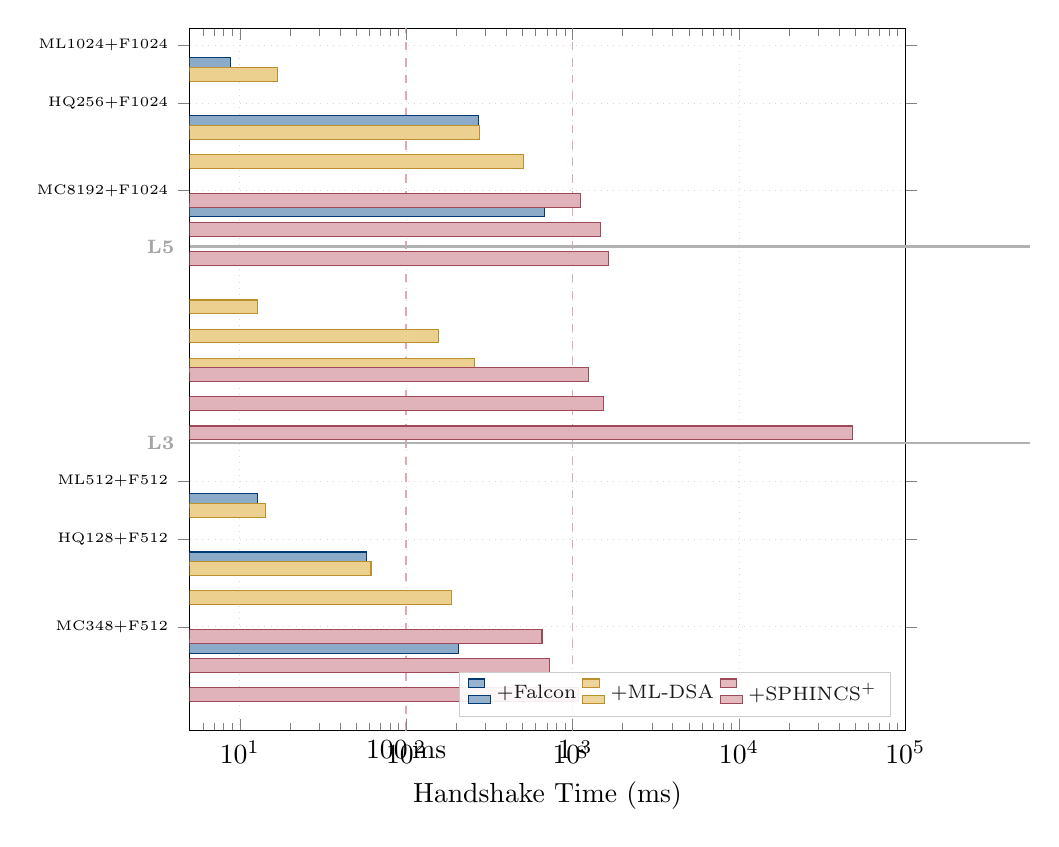
\begin{tikzpicture}
\begin{axis}[
  xbar,
  width=0.88\textwidth,
  height=10.5cm,
  bar width=5pt,
  xlabel={Handshake Time (ms)},
  xmode=log, log basis x=10,
  xmin=5, xmax=100000,
  symbolic y coords={%
    MC348+SP128,HQ128+SP128,ML512+SP128,MC348+F512,MC348+DSA44,%
    HQ128+DSA44,HQ128+F512,ML512+DSA44,ML512+F512,%
    MC460+SP192,HQ192+SP192,ML768+SP192,%
    MC460+DSA65,HQ192+DSA65,ML768+DSA65,%
    MC8192+SP256,HQ256+SP256,ML1024+SP256,%
    MC8192+F1024,MC8192+DSA87,HQ256+DSA87,HQ256+F1024,%
    ML1024+DSA87,ML1024+F1024%
  },
  ytick=data,
  y tick label style={font=\tiny},
  enlarge y limits=0.025,
  grid=major, grid style={dotted, gray!30},
  extra x ticks={100,1000},
  extra x tick labels={\SI{100}{ms},\SI{1}{s}},
  extra x tick style={grid=major, grid style={dashed, ptrose!50, line width=0.6pt}},
  legend style={at={(0.98,0.02)}, anchor=south east, font=\scriptsize,
    legend columns=3, fill=white, fill opacity=0.9, draw=gray!40},
]
% Falcon suites (ptblue)
\addplot[fill=ptblue!45, draw=ptblue!85!black] coordinates {
  (12.80,ML512+F512) (57.80,HQ128+F512) (206.1,MC348+F512)
  (8.75,ML1024+F1024) (271.7,HQ256+F1024) (678.4,MC8192+F1024)
};
\addlegendentry{+Falcon}
% ML-DSA suites (ptgold)
\addplot[fill=ptgold!55, draw=ptgold!85!black] coordinates {
  (14.34,ML512+DSA44) (61.43,HQ128+DSA44) (187.5,MC348+DSA44)
  (12.71,ML768+DSA65) (155.8,HQ192+DSA65) (257.4,MC460+DSA65)
  (16.78,ML1024+DSA87) (276.1,HQ256+DSA87) (505.3,MC8192+DSA87)
};
\addlegendentry{+ML-DSA}
% SPHINCS+ suites (ptrose)
\addplot[fill=ptrose!45, draw=ptrose!85!black] coordinates {
  (655.1,ML512+SP128) (722.8,HQ128+SP128) (1079.9,MC348+SP128)
  (1249.5,ML768+SP192) (1537.0,HQ192+SP192) (48186,MC460+SP192)
  (1110.2,ML1024+SP256) (1469.9,HQ256+SP256) (1650.8,MC8192+SP256)
};
\addlegendentry{+SPHINCS$^+$}
\end{axis}
% Level separator annotations
\draw[thick, gray!60] ([yshift=3.65cm]current axis.south west) -- ++(0.88\textwidth,0);
\node[font=\scriptsize\bfseries, text=gray!70, anchor=east]
  at ([yshift=3.65cm, xshift=-2pt]current axis.south west) {L3};
\draw[thick, gray!60] ([yshift=6.15cm]current axis.south west) -- ++(0.88\textwidth,0);
\node[font=\scriptsize\bfseries, text=gray!70, anchor=east]
  at ([yshift=6.15cm, xshift=-2pt]current axis.south west) {L5};
\end{tikzpicture}
\caption{All 24 suites ranked by handshake time, colour-coded by SIG family
  (Falcon: \textcolor{ptblue}{blue}, ML-DSA: \textcolor{ptgold}{gold},
  SPHINCS$^+$: \textcolor{ptrose}{rose}).
  SPHINCS$^+$ suites cluster at the slow end ($>$\SI{655}{ms}).
  Dashed lines mark the \SI{100}{ms} and \SI{1}{s} deadlines.}
\label{fig:suite_bars}
\end{figure*}

%% ----------------------------------------------------------------
%%  FIGURE 2 — Three-Metric Bubble Plot: BW × HS Time × Energy
%% ----------------------------------------------------------------
\begin{figure}[t]
\centering
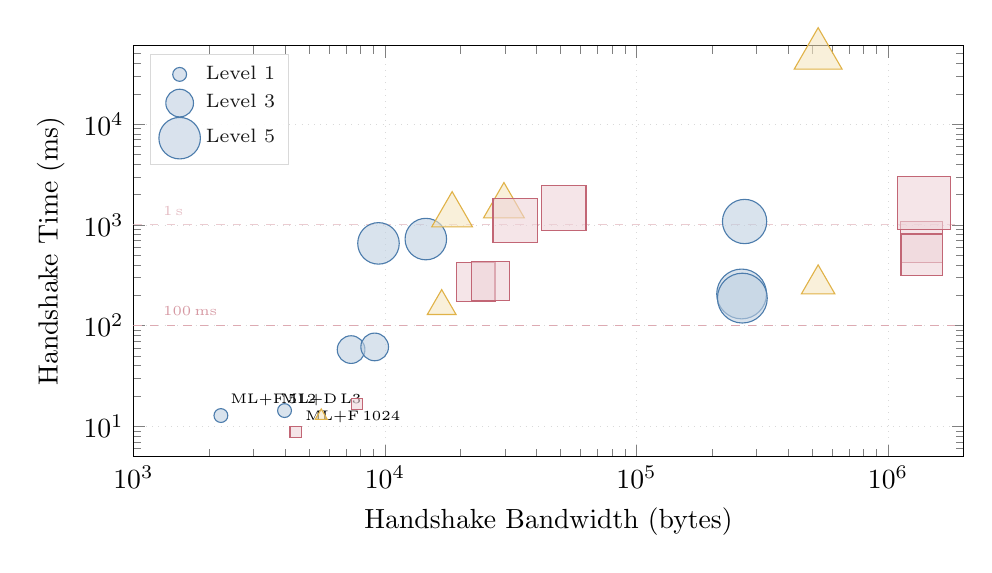
\begin{tikzpicture}
\begin{axis}[
  width=\columnwidth,
  height=6.8cm,
  xlabel={Handshake Bandwidth (bytes)},
  ylabel={Handshake Time (ms)},
  xmode=log, ymode=log,
  log basis x=10, log basis y=10,
  xmin=1000, xmax=2000000,
  ymin=5, ymax=60000,
  grid=major, grid style={dotted, gray!30},
  legend style={at={(0.02,0.98)}, anchor=north west, font=\scriptsize,
    legend columns=1, fill=white, fill opacity=0.9, draw=gray!30},
]
% --- L1 suites (circles) ---
\addplot[only marks, mark=*, color=ptblue!70, fill=ptblue!25,
  fill opacity=0.6, mark size=2.5pt]
  coordinates {(2227,12.80) (3988,14.34)};
\addplot[only marks, mark=*, color=ptblue!70, fill=ptblue!25,
  fill opacity=0.6, mark size=5pt]
  coordinates {(7335,57.80) (9102,61.43)};
\addplot[only marks, mark=*, color=ptblue!70, fill=ptblue!25,
  fill opacity=0.6, mark size=7.5pt]
  coordinates {(9424,655.1) (14538,722.8)};
\addplot[only marks, mark=*, color=ptblue!70, fill=ptblue!25,
  fill opacity=0.6, mark size=9pt]
  coordinates {(261870,206.1) (263636,187.5)};
\addplot[only marks, mark=*, color=ptblue!70, fill=ptblue!25,
  fill opacity=0.6, mark size=8pt]
  coordinates {(269072,1079.9)};
\addlegendentry{Level 1}
% --- L3 suites (triangles) ---
\addplot[only marks, mark=triangle*, color=ptgold!90, fill=ptgold!30,
  fill opacity=0.6, mark size=2.5pt]
  coordinates {(5581,12.71)};
\addplot[only marks, mark=triangle*, color=ptgold!90, fill=ptgold!30,
  fill opacity=0.6, mark size=6pt]
  coordinates {(16809,155.8)};
\addplot[only marks, mark=triangle*, color=ptgold!90, fill=ptgold!30,
  fill opacity=0.6, mark size=7pt]
  coordinates {(527625,257.4)};
\addplot[only marks, mark=triangle*, color=ptgold!90, fill=ptgold!30,
  fill opacity=0.6, mark size=8.5pt]
  coordinates {(18496,1249.5) (29724,1537.0)};
\addplot[only marks, mark=triangle*, color=ptgold!90, fill=ptgold!30,
  fill opacity=0.6, mark size=10pt]
  coordinates {(527625,48186)};
\addlegendentry{Level 3}
% --- L5 suites (squares) ---
\addplot[only marks, mark=square*, color=ptrose!90, fill=ptrose!25,
  fill opacity=0.6, mark size=2pt]
  coordinates {(4410,8.75) (7763,16.78)};
\addplot[only marks, mark=square*, color=ptrose!90, fill=ptrose!25,
  fill opacity=0.6, mark size=7pt]
  coordinates {(22943,271.7) (26293,276.1)};
\addplot[only marks, mark=square*, color=ptrose!90, fill=ptrose!25,
  fill opacity=0.6, mark size=8pt]
  coordinates {(32928,1110.2) (51458,1469.9)};
\addplot[only marks, mark=square*, color=ptrose!90, fill=ptrose!25,
  fill opacity=0.6, mark size=7.5pt]
  coordinates {(1359303,678.4) (1362659,505.3)};
\addplot[only marks, mark=square*, color=ptrose!90, fill=ptrose!25,
  fill opacity=0.6, mark size=9.5pt]
  coordinates {(1387824,1650.8)};
\addlegendentry{Level 5}
% Key-suite labels
\node[font=\tiny, anchor=south west] at (axis cs:2227,12.80) {ML+F\,512};
\node[font=\tiny, anchor=south west] at (axis cs:4410,8.75) {ML+F\,1024};
\node[font=\tiny, anchor=south]      at (axis cs:5581,12.71) {ML+D\,L3};
% Deadline lines
\draw[dashed, ptrose!50, thin] (axis cs:1000,100) -- (axis cs:2000000,100);
\node[font=\tiny, text=ptrose!60, anchor=south west] at (axis cs:1200,100)
  {\SI{100}{ms}};
\draw[dashed, ptrose!30, thin] (axis cs:1000,1000) -- (axis cs:2000000,1000);
\node[font=\tiny, text=ptrose!40, anchor=south west] at (axis cs:1200,1000)
  {\SI{1}{s}};
\end{axis}
\end{tikzpicture}
\caption{Three-metric bubble plot: bandwidth~(x) $\times$ handshake time~(y)
  $\times$ energy~(bubble area).
  Ideal suites cluster at the bottom-left with small bubbles.
  ML-KEM+Falcon/DSA form a tight cluster at $<$\SI{17}{ms},
  $<$\SI{8}{KB}, $<$\SI{60}{mJ}.}
\label{fig:suite_bubble}
\end{figure}

%% ----------------------------------------------------------------
%%  FIGURE 3 — Crypto vs Protocol Overhead (Stacked Bars)
%% ----------------------------------------------------------------
\begin{figure}[t]
\centering
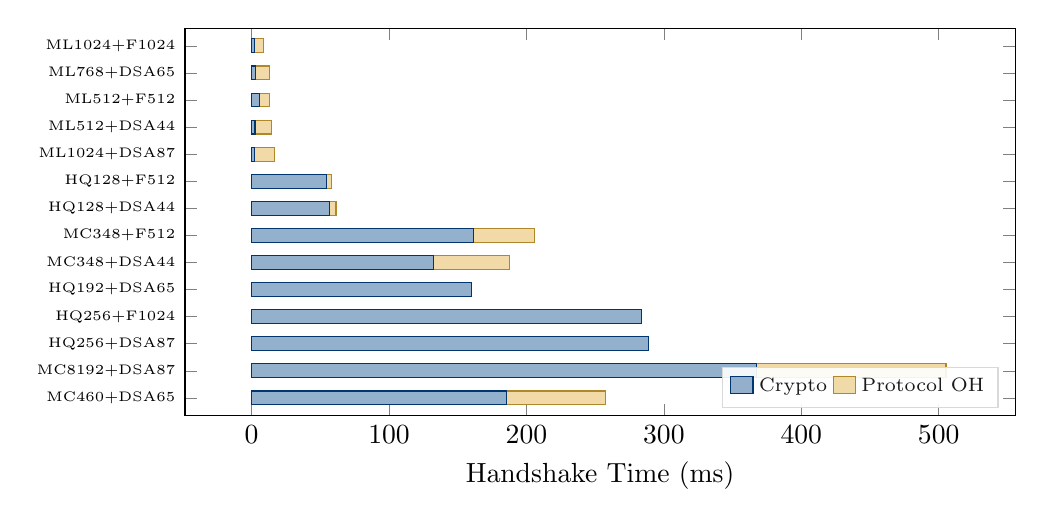
\begin{tikzpicture}
\begin{axis}[
  xbar stacked,
  width=\columnwidth,
  height=6.5cm,
  xlabel={Handshake Time (ms)},
  symbolic y coords={%
    MC460+DSA65,MC8192+DSA87,HQ256+DSA87,HQ256+F1024,HQ192+DSA65,%
    MC348+DSA44,MC348+F512,%
    HQ128+DSA44,HQ128+F512,%
    ML1024+DSA87,ML512+DSA44,ML512+F512,ML768+DSA65,ML1024+F1024%
  },
  ytick=data,
  y tick label style={font=\tiny},
  legend style={at={(0.98,0.02)}, anchor=south east, font=\scriptsize,
    legend columns=2, fill=white, fill opacity=0.9, draw=gray!30},
  bar width=5pt,
  enlarge y limits=0.05,
  every axis plot/.append style={fill opacity=0.85},
]
% Crypto time
\addplot[fill=ptblue!50, draw=ptblue!80!black] coordinates {
  (1.82,ML1024+F1024)  (2.71,ML768+DSA65)  (5.69,ML512+F512)
  (2.45,ML512+DSA44)   (2.25,ML1024+DSA87)
  (54.30,HQ128+F512)   (56.50,HQ128+DSA44)
  (161.4,MC348+F512)   (132.3,MC348+DSA44)
  (159.9,HQ192+DSA65)  (283.7,HQ256+F1024)
  (288.9,HQ256+DSA87)  (367.3,MC8192+DSA87)
  (185.4,MC460+DSA65)
};
\addlegendentry{Crypto}
% Protocol overhead = T_HS - T_crypto
\addplot[fill=ptgold!50, draw=ptgold!80!black] coordinates {
  (6.93,ML1024+F1024)  (10.00,ML768+DSA65)  (7.11,ML512+F512)
  (11.89,ML512+DSA44)  (14.53,ML1024+DSA87)
  (3.50,HQ128+F512)    (4.93,HQ128+DSA44)
  (44.7,MC348+F512)    (55.2,MC348+DSA44)
  (0,HQ192+DSA65)      (0,HQ256+F1024)
  (0,HQ256+DSA87)      (138.0,MC8192+DSA87)
  (72.0,MC460+DSA65)
};
\addlegendentry{Protocol OH}
\end{axis}
\end{tikzpicture}
\caption{Crypto vs.\ protocol overhead for viable and marginal suites
  (SPHINCS$^+$ omitted: $>$98\% crypto-dominated).
  For ML-KEM suites, protocol overhead (Python, HKDF, socket I/O) accounts for
  40--85\% of $T_\text{HS}$; for HQC/McEliece, crypto dominates at $>$70\%.}
\label{fig:suite_overhead}
\end{figure}

%% ----------------------------------------------------------------
%%  FIGURE 4 — Energy vs HS Time Scatter with Viability Zones
%% ----------------------------------------------------------------
\begin{figure}[t]
\centering
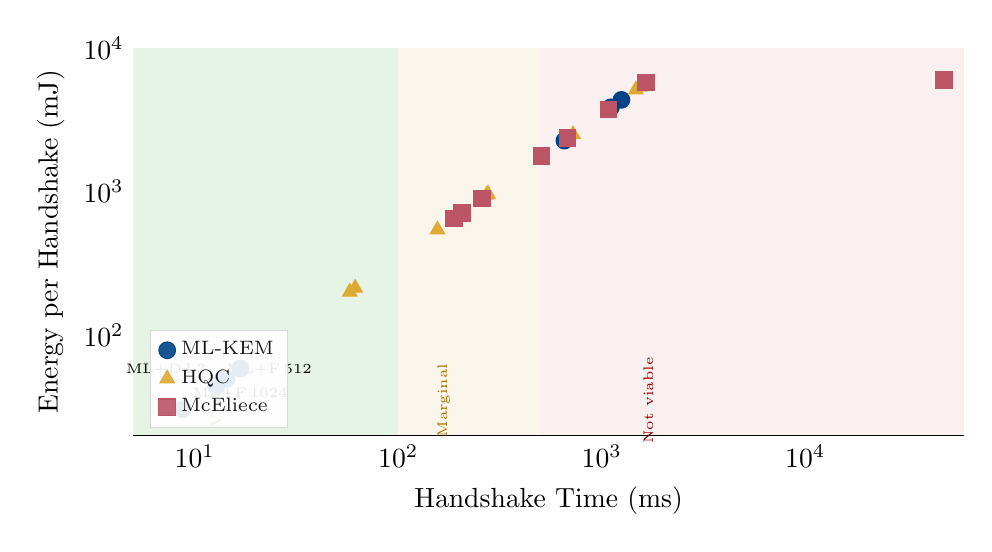
\begin{tikzpicture}
\begin{axis}[
  width=\columnwidth,
  height=6.5cm,
  xlabel={Handshake Time (ms)},
  ylabel={Energy per Handshake (mJ)},
  xmode=log, ymode=log,
  log basis x=10, log basis y=10,
  xmin=5, xmax=60000,
  ymin=20, ymax=10000,
  grid=major, grid style={dotted, gray!30},
  legend style={at={(0.02,0.02)}, anchor=south west, font=\scriptsize,
    legend columns=1, fill=white, fill opacity=0.9, draw=gray!30},
  clip=false,
]
% Viability zone shading
\fill[viable!10] (axis cs:5,20) rectangle (axis cs:100,10000);
\fill[marginal!8] (axis cs:100,20) rectangle (axis cs:500,10000);
\fill[notviable!6] (axis cs:500,20) rectangle (axis cs:60000,10000);
% Zone labels
\node[font=\tiny, text=viable!80!black, rotate=90, anchor=south]
  at (axis cs:15,35) {Viable};
\node[font=\tiny, text=marginal!80!black, rotate=90, anchor=south]
  at (axis cs:200,35) {Marginal};
\node[font=\tiny, text=notviable!80!black, rotate=90, anchor=south]
  at (axis cs:2000,35) {Not viable};
% ML-KEM family
\addplot[only marks, mark=*, color=ptblue, mark size=3pt] coordinates {
  (12.80, 44.3)  (14.34, 49.6)  (655.1, 2268)
  (12.71, 44.3)  (1249.5, 4362)
  (8.75, 30.5)   (16.78, 58.5)  (1110.2, 3873)
};
\addlegendentry{ML-KEM}
% HQC family
\addplot[only marks, mark=triangle*, color=ptgold, mark size=3pt] coordinates {
  (57.80, 200)   (61.43, 213)   (722.8, 2502)
  (155.8, 543)   (1537.0, 5364)
  (271.7, 947)   (276.1, 963)   (1469.9, 5128)
};
\addlegendentry{HQC}
% McEliece family
\addplot[only marks, mark=square*, color=ptrose, mark size=3pt] coordinates {
  (206.1, 713)   (187.5, 649)   (1079.9, 3739)
  (257.4, 897)   (48186, 6000)
  (678.4, 2367)  (505.3, 1763)  (1650.8, 5759)
};
\addlegendentry{McEliece}
% Best-suite labels
\node[font=\tiny, anchor=south west] at (axis cs:8.75,30.5) {ML+F\,1024};
\node[font=\tiny, anchor=south west] at (axis cs:12.80,44.3) {ML+F\,512};
\node[font=\tiny, anchor=south east] at (axis cs:12.71,44.3) {ML+D\,L3};
\end{axis}
\end{tikzpicture}
\caption{Energy vs.\ handshake time with viability zones.
  All six viable suites ($<$\SI{100}{ms}) cluster in the green zone and use
  ML-KEM; SPHINCS$^+$ pushes every KEM into the red zone.
  Energy and time are strongly correlated ($R^2>0.95$).}
\label{fig:suite_energy}
\end{figure}

%% ----------------------------------------------------------------
%%  FIGURE 5 — Slowdown Factor ρ by KEM×SIG (Grouped Bars)
%% ----------------------------------------------------------------
\begin{figure}[t]
\centering
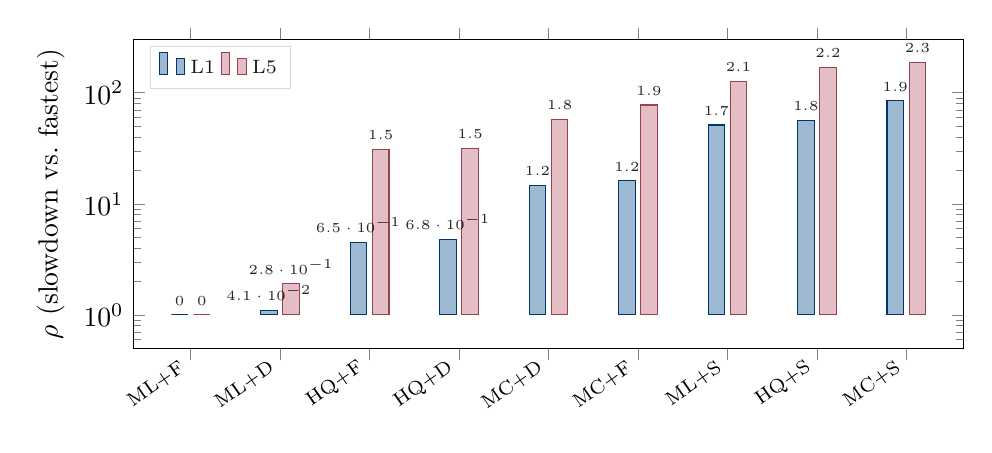
\begin{tikzpicture}
\begin{axis}[
  ybar,
  width=\columnwidth,
  height=5.5cm,
  bar width=6pt,
  ylabel={$\rho$ (slowdown vs.\ fastest)},
  ymode=log, log basis y=10,
  ymin=0.5, ymax=300,
  symbolic x coords={ML+F,ML+D,HQ+F,HQ+D,MC+D,MC+F,ML+S,HQ+S,MC+S},
  xtick=data,
  x tick label style={rotate=35, anchor=east, font=\scriptsize},
  legend style={at={(0.02,0.98)}, anchor=north west, font=\scriptsize,
    legend columns=2, fill=white, fill opacity=0.9, draw=gray!30},
  every axis plot/.append style={fill opacity=0.85},
  enlarge x limits=0.08,
  nodes near coords,
  nodes near coords style={font=\tiny, /pgf/number format/precision=1},
]
% L1
\addplot[fill=ptblue!45, draw=ptblue!80!black] coordinates {
  (ML+F,1.0)  (ML+D,1.1)  (HQ+F,4.5)  (HQ+D,4.8)
  (MC+D,14.6) (MC+F,16.1) (ML+S,51.2) (HQ+S,56.5) (MC+S,84.4)
};
\addlegendentry{L1}
% L5
\addplot[fill=ptrose!45, draw=ptrose!80!black] coordinates {
  (ML+F,1.0)  (ML+D,1.9)  (HQ+F,31.0) (HQ+D,31.6)
  (MC+D,57.8) (MC+F,77.5) (ML+S,126.9)(HQ+S,168.1)(MC+S,188.8)
};
\addlegendentry{L5}
\end{axis}
\end{tikzpicture}
\caption{Slowdown factor $\rho$ at L1 and L5.
  ML-KEM+Falcon is the $1.0\times$ baseline; SPHINCS$^+$ suites incur
  50--189$\times$ slowdown.  Even HQC+Falcon at L5 is $31\times$ slower.}
\label{fig:suite_rho}
\end{figure}

%% ----------------------------------------------------------------
%%  FIGURE 6 — Bandwidth Composition: KEM vs SIG (Stacked Bars)
%% ----------------------------------------------------------------
\begin{figure}[t]
\centering
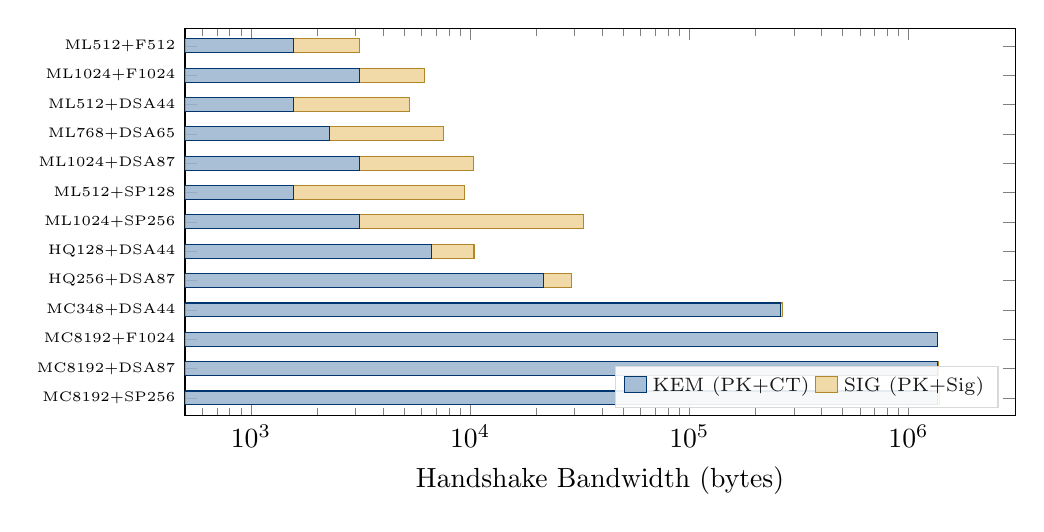
\begin{tikzpicture}
\begin{axis}[
  xbar stacked,
  width=\columnwidth,
  height=6.5cm,
  xmode=log, log basis x=10,
  xlabel={Handshake Bandwidth (bytes)},
  xmin=500,
  symbolic y coords={%
    MC8192+SP256,MC8192+DSA87,MC8192+F1024,%
    MC348+DSA44,%
    HQ256+DSA87,HQ128+DSA44,%
    ML1024+SP256,ML512+SP128,%
    ML1024+DSA87,ML768+DSA65,ML512+DSA44,%
    ML1024+F1024,ML512+F512%
  },
  ytick=data,
  y tick label style={font=\tiny},
  legend style={at={(0.98,0.02)}, anchor=south east, font=\scriptsize,
    legend columns=2, fill=white, fill opacity=0.9, draw=gray!30},
  bar width=5pt,
  enlarge y limits=0.05,
  every axis plot/.append style={fill opacity=0.85},
]
% KEM contribution (PK + CT)
\addplot[fill=ptblue!40, draw=ptblue!80!black] coordinates {
  (1568,ML512+F512)     (1568,ML512+DSA44)    (1568,ML512+SP128)
  (2272,ML768+DSA65)
  (3136,ML1024+F1024)   (3136,ML1024+DSA87)   (3136,ML1024+SP256)
  (6682,HQ128+DSA44)
  (21666,HQ256+DSA87)
  (261216,MC348+DSA44)
  (1358032,MC8192+F1024)(1358032,MC8192+DSA87)(1358032,MC8192+SP256)
};
\addlegendentry{KEM (PK+CT)}
% SIG contribution (PK + Sig)
\addplot[fill=ptgold!50, draw=ptgold!80!black] coordinates {
  (1551,ML512+F512)     (3732,ML512+DSA44)    (7888,ML512+SP128)
  (5261,ML768+DSA65)
  (3060,ML1024+F1024)   (7219,ML1024+DSA87)   (29856,ML1024+SP256)
  (3732,HQ128+DSA44)
  (7219,HQ256+DSA87)
  (3732,MC348+DSA44)
  (3060,MC8192+F1024)   (7219,MC8192+DSA87)   (29856,MC8192+SP256)
};
\addlegendentry{SIG (PK+Sig)}
\end{axis}
\end{tikzpicture}
\caption{Bandwidth composition: KEM (PK+ciphertext) vs.\ SIG (PK+signature).
  ML-KEM suites split roughly equally; McEliece dominates at $>$99\% of
  total BW due to 261\,KB--1.36\,MB public keys.
  SPHINCS$^+$ adds 7.9--29.9\,KB but is dwarfed by McEliece's KEM payload.}
\label{fig:suite_bw}
\end{figure}

%% ----------------------------------------------------------------
%%  Analysis Text
%% ----------------------------------------------------------------

\subsubsection{Crypto vs.\ Protocol Overhead}
Fig.~\ref{fig:suite_overhead} decomposes $T_\text{HS}$ into
cryptographic and protocol overhead for viable and marginal suites.
For ML-KEM suites, the cryptographic component is surprisingly small:
ML1024+F1024 spends only \SI{1.82}{ms} (20.8\%) on crypto;
ML512+DSA44 spends \SI{2.45}{ms} (17.1\%).  Protocol overhead---Python
interpreter, HKDF derivation, socket I/O, session bookkeeping---accounts
for 40--85\% of total handshake time.  This implies that a
\emph{C/Rust rewrite of the handshake controller} could cut ML-KEM
suite latency by $2$--$5\times$, potentially pushing even HQC-128
suites below the \SI{100}{ms} threshold.

In contrast, HQC and McEliece suites are crypto-dominated: HQC-128+F512
spends 93.9\% on crypto (\SI{54.3}{ms} of \SI{57.8}{ms}), and
McEliece-348+F512 spends 78.3\% (\SI{161.4}{ms} of \SI{206.1}{ms}).
For these families, protocol optimization yields diminishing returns;
algorithmic improvements to the KEM itself are needed.

\subsubsection{Bandwidth Constraints}
Fig.~\ref{fig:suite_bw} reveals the bandwidth composition.  ML-KEM
suites require 2--9\,KB total handshake bandwidth, comfortably within
a single UDP datagram.  McEliece suites explode to
261\,KB (MC348) and 1.36\,MB (MC8192), where the KEM public key
alone exceeds most MTU-aware fragmentation budgets.  MC8192's
1.36\,MB handshake payload would require ${\sim}1{,}000$ UDP
fragments at standard 1400-byte payloads, introducing reassembly
latency that contributes to its \SI{505}{ms}--\SI{1651}{ms} observed
handshake times.

\subsubsection{SPHINCS$^+$ Disqualification}
SPHINCS$^+$ renders \emph{every} suite non-viable regardless of KEM
choice (Table~\ref{tab:suite_decision}).  Even the fastest combination,
ML-KEM-512+SP128 at \SI{655}{ms}, exceeds the \SI{100}{ms}
viability threshold by $6.5\times$.  The worst case, MC460+SP192 at
\SI{48186}{ms} (\SI{48.2}{s}), constitutes a complete timeout---this
confirms the MDEAS cross-axis constraint that eliminates SPHINCS$^+$
from the viable operating region (Sec.~\ref{sec:scheduler_analysis}).

\subsubsection{Structural Findings}
Three structural findings emerge from the 24-suite evaluation and are
visualized in Figs.~\ref{fig:suite_bars}--\ref{fig:suite_rho}:

\begin{enumerate}
\item \textbf{ML-KEM is the only KEM family viable at all levels.}
  ML-KEM suites achieve sub-\SI{17}{ms} with Falcon or ML-DSA at
  L1, L3, and L5.  HQC enters the marginal zone at L3
  (\SI{156}{ms}) and L5 (\SI{272}{ms}).  McEliece exceeds
  \SI{187}{ms} even at L1.

\item \textbf{SPHINCS$^+$ is a universal disqualifier.}
  All 9 SPHINCS$^+$ suites exceed \SI{655}{ms}.  The signing
  cost alone ($>$\SI{640}{ms} at L1) exceeds the entire
  handshake budget.

\item \textbf{McEliece L5 exceeds all deadlines.}
  MC8192+DSA87 at \SI{505}{ms} and MC8192+F1024 at \SI{678}{ms}
  both exceed the \SI{500}{ms} ``marginal'' boundary.  Combined with
  1.36\,MB bandwidth, McEliece-8192 is structurally incompatible with
  real-time UAV links.
\end{enumerate}

\noindent
These findings directly inform MDEAS policy: the scheduler restricts
the viable operating region to ML-KEM$\,\times\,$(Falcon$\mid$ML-DSA)
suites, reducing the 24-suite space to 7~candidates (6~viable +
McEliece-348+DSA44 at \SI{187.5}{ms} as an extended-rekey fallback).


\end{document}
